\documentclass[openany]{book}

\usepackage{fancyhdr} % For style
\usepackage{geometry} % For margins
\usepackage{tocloft} % For TOC dots
\usepackage{multicol} % For multiple columns
\usepackage{graphicx} % For incorporating pictures

\geometry{margin=1in, headsep=30pt, top=1.5in, left=.75in, right=.75in}
\pagestyle{fancy}

\renewcommand{\cftchapleader}{\cftdotfill{\cftdotsep}}

% "recipes.sty" package starts here:
\newcommand{\recipe}[1]{%
    \newpage
    \ichapter{#1}
    \chead{\Huge \bf{#1}}}%

\newcommand{\preptime}[1]{%
    \lhead{Prep time: #1}}

\newcommand{\cooktime}[1]{%
    \rhead{Cook time: #1}}

\newcommand{\ingredients}[1][\textbf{\Large\emph{Ingredients}}]{%
    \begin{center} \emph{#1} \end{center}}

\newcommand{\instructions}[1][
    \textbf{\Large\emph{Instructions}}]{%
    \begin{center}
    \emph{#1}
    \end{center}}%

\newcommand{\temp}[1]{%
    $#1^\circ$F}

% Cover Page
\title{Recipes}
\author{Brad Hall}
\date{}


\newcommand\ichapter[1]{%
  \refstepcounter{chapter}%
  \addcontentsline{toc}{chapter}{\protect\numberline{\thechapter}#1}%
  \sectionmark{#1}}

\begin{document}
\maketitle
\tableofcontents
\newpage

%%% BEEF STEW %%%

\recipe{Beef Stew}
\preptime{15 min}
\cooktime{2 hrs 40 mins}

\begin{multicols}{2}
\ingredients
\begin{itemize}
    \item 2.4lb chuck beef (cut into 3.5 cm/1.5'' cubes)
    \item 1 tsp each salt and pepper
    \item 3 tbsp olive oil (divided)
    \item 1 large onion (cut finely)
    \item 4 garlic cloves (minced)
    \item 3 carrots (cut into 2.5 cm/1'' pieces)
    \item 2 celery stalks (cut into 2.5 cm/1'' pieces)
    \item 1/3 cup flour
    \item 5 cups beef broth
    \item 2 tsp Worcestershire sauce
    \item 2 tbsp tomato paste
    \item 400 g/14 oz baby potatos (halved or quartered)
    \item More salt and pepper (to taste)
\end{itemize}

\vfill\null
\columnbreak

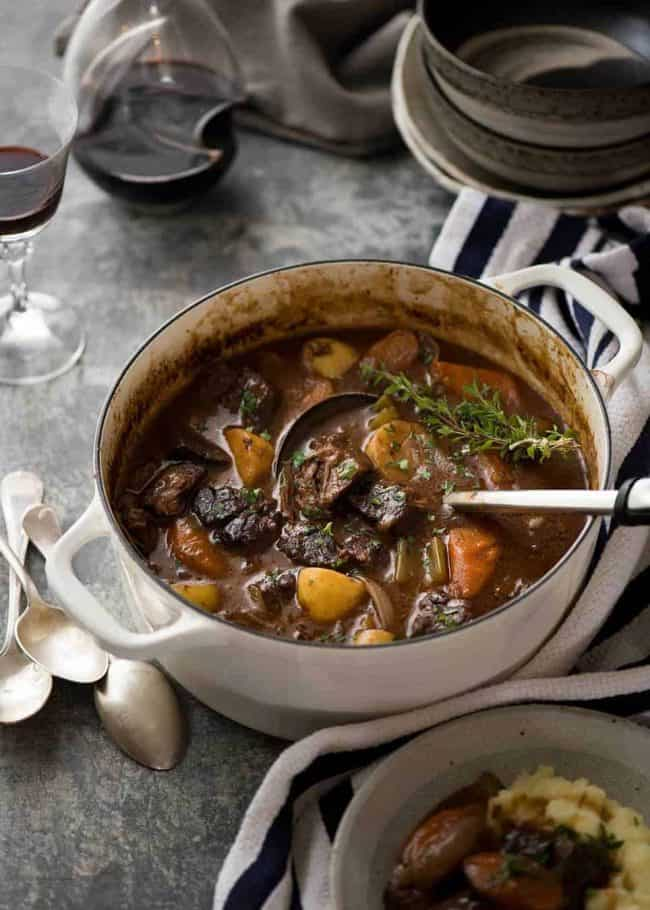
\includegraphics[height=8.75cm, width=7.5cm]{Pictures/Beef_Stew.jpg}
\end{multicols}

\instructions
\begin{enumerate}
    \item Sprinkle beef with salt and pepper.
    \item Heat 1 1/2 tbsp oil in a large, heavy based casserole pot over high heat until just starting to smoke.
    \item Add 1/3 of the beef and brown aggressively all over - about 4 minutes. Remove to bowl, repeat with remaining beef, adding more oil if required.
    \item Turn down heat to medium high. Add 1 tbsp oil if required. Add onion and garlic, cook for 2 minutes until onion is softened slightly and golden on the edge.
    \item Add carrot and celery, stir for 1 minute to coat in flavours.
    \item Sprinkle flour evenly across surface, then stir to coat.
    \item Add broth, tomato paste and Worcestershire sauce. Stir to dissolve tomato paste and flour into liquid.
    \item Add cooked beef (including any juices) and potato. Stir. Water level should almost fully cover everything, if not, add a touch of water.
    \item Bring to simmer, then adjust heat to low/medium low so it's simmering gently.
    \item Cover and cook for 1 hour 45 minutes or until beef is pretty tender (check with 2 forks at 1.5 hrs).
    \item Remove lid and simmer for further 30 minutes or until sauce reduces slightly. It should be like a thin gravy and beef should now be very tender.
    \item Season to taste with salt and pepper. 
    \item Serve over creamy mashed potato.
\end{enumerate}

%%% MEATLOAF %%%

\recipe{Meatloaf}
\preptime{10 min}
\cooktime{1 hr}

\begin{multicols}{2}
\ingredients
\begin{itemize}
    \item 1 1/2 lb ground beef
    \item 1 egg
    \item 1 onion (chopped)
    \item 1 cup milk
    \item 1 cup dried bread crumbs
    \item salt and pepper 
    \item 2 tbsp brown sugar
    \item 2 tbsp prepared mustard
    \item 1/3 cup ketchup
\end{itemize}

\vfill\null
\columnbreak

\hspace{-1cm}
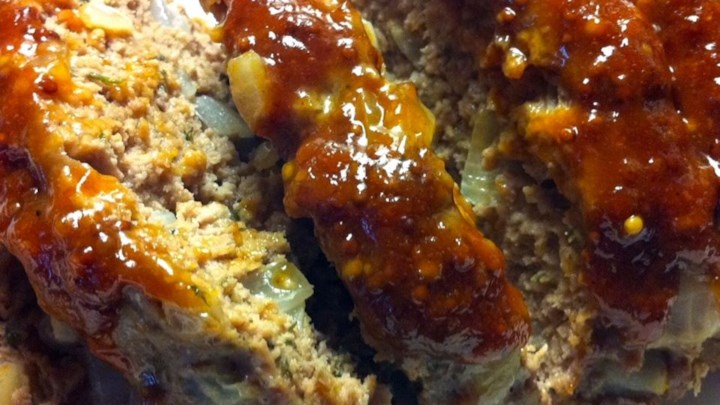
\includegraphics[height=6.25cm, width=8.5cm]{Pictures/Meatloaf.jpg}
\end{multicols}

\instructions
\begin{enumerate}
    \item Preheat oven to \temp{350}.
    \item In a large bowl, combine the beef, egg, onion, milk and bread crumbs. Season with salt and pepper to taste and place in a lightly greased 5x9 inch loaf pan (or form into a loaf and place in a lightly greased 9x13 inch baking dish).
    \item In a separate small bowl, combine the brown sugar, mustard and ketchup. Mix well and pour over the meatloaf.
    \item Bake at \temp{350} for 1 hour.
\end{enumerate}

%%% CHICKEN PARMESAN %%%

\recipe{Chicken Parmesan}
\preptime{10 min}
\cooktime{25 min}

\begin{multicols}{2}
\ingredients
\begin{itemize}
	\item 4 skinless boneless chicken breast halves
	\item 1/2 cup flour
	\item 2 eggs
	\item 2/3 cup Panko bread crumbs
	\item 2/3 cup Italian Seasoning bread crumbs
	\item 1/3 cup grated parmesan cheese
	\item 2 tbsp parsley
	\item 4 tbsp oil (or as needed)
	\item 24 oz marinara sauce
	\item 1 cup mozzarella cheese shredded
	\item 1/4 cup shredded Parmesan cheese
	\item basil \& parsley fresh, chopped
\end{itemize}

\vfill\null
\columnbreak

\hspace{-1.5cm}
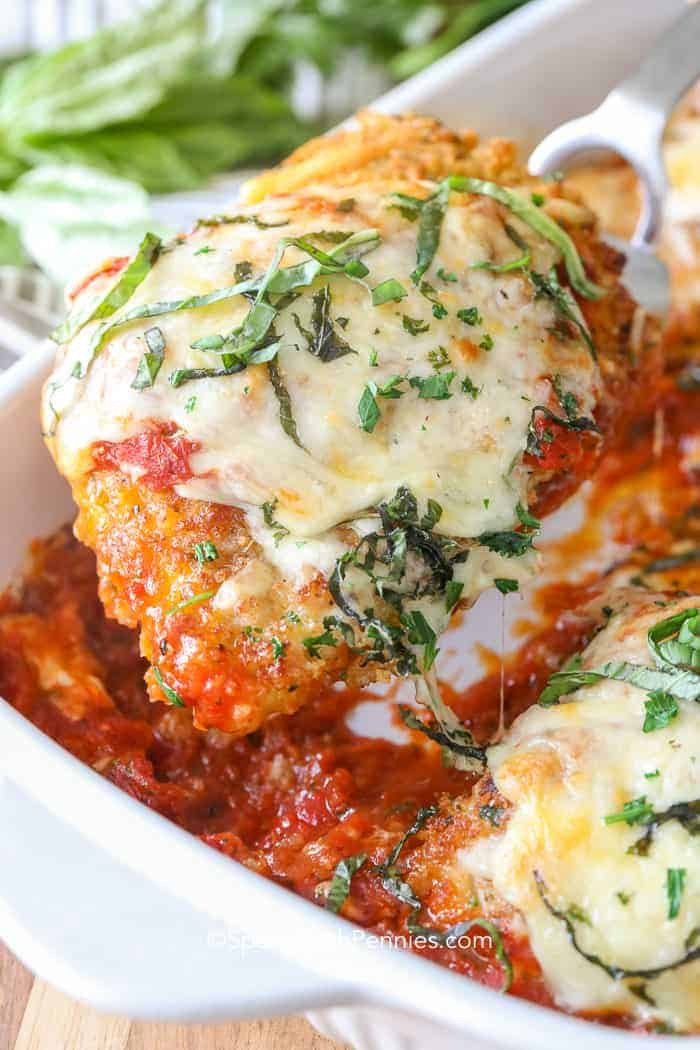
\includegraphics[height=8.25cm, width=9.25cm]{Pictures/Chicken_Parmesan.jpg}
\end{multicols}

\instructions
\begin{enumerate}
    \item Preheat oven to \temp{425}.
    \item Place flour in shallow dish. Place the eggs in a second dish (and beat with a fork).
    \item Combine Panko, Italian crumbs, grated parmesan, 2 tablespoons fresh parsley, salt and pepper to taste in a third shallow dish.
    \item Pound chicken breasts to 1/2 inch thick (if they're very large you can cut them in half).
    \item Dip chicken into flour and shake to remove any excess. Dip chicken in beaten eggs \& then into bread crumb mixture (press to adhere).
    \item Preheat oil in a large pan. Brown chicken on each side, about 4 minutes per side or until golden (it does not need to cook through as it will continue to cook in the oven).
    \item Place 1 1/2 cups of marinara sauce in the bottom of a 9x13 dish. Add browned chicken. Top each piece with a couple tablespoons of marinara sauce, mozzarella and parmesan.
        8. Bake 20-25 minutes or until golden and bubbly and chicken reaches \temp{165}. Sprinkle with fresh herbs and serve over pasta.
\end{enumerate}

%%% CHILI %%%

\recipe{Chili}
\preptime{5 mins}
\cooktime{25 mins}

\begin{multicols}{2}
\ingredients
\begin{itemize}
    \item 1 tbsp olive oil
    \item 1 medium yellow onion (diced)
    \item 1lb 90\% lean ground beef
    \item 2 1/2 tablespoons chili powder
    \item 2 tbsp ground cumin
    \item 2 tbsp granulated sugar
    \item 2 tbsp tomato paste
    \item 1 tbsp garlic powder
    \item 1 1/2 tsp salt
    \item 1/2 tsp ground black pepper
    \item 1 1/2 cups beef broth
    \item 1 (15 oz) can petite diced tomatoes
    \item 1 (8 oz) can tomato sauce
\end{itemize}

\vfill\null
\columnbreak

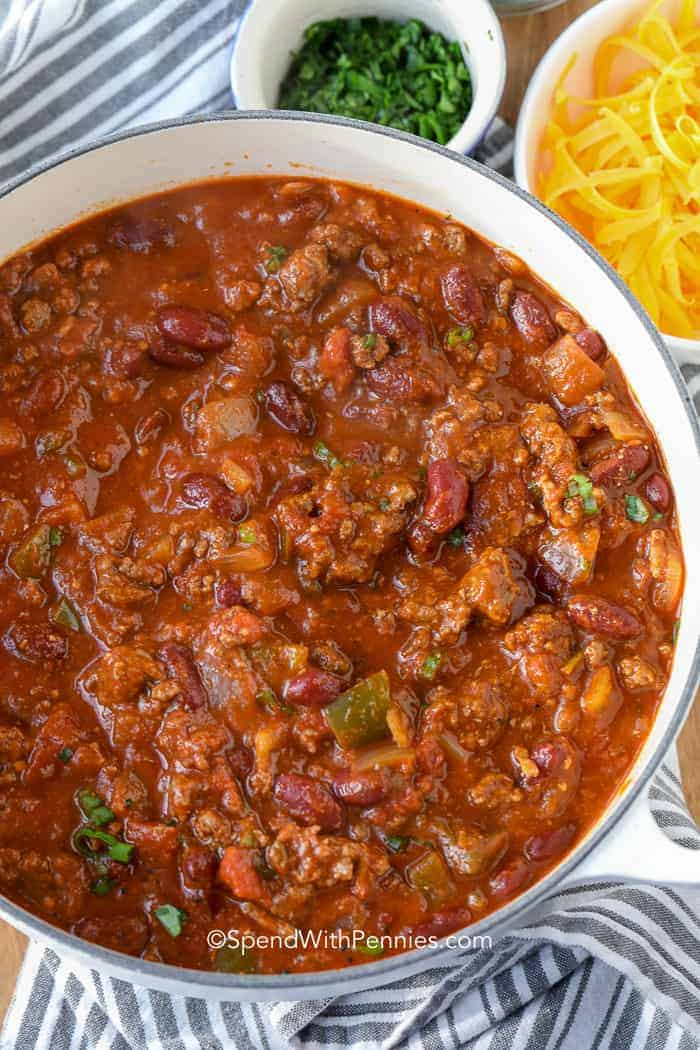
\includegraphics[height=8.75cm, width=7.5cm]{Pictures/Chili.jpg}
\end{multicols}

\instructions
\begin{enumerate}
    \item Add the olive oil to a large soup pot and place it over medium-high heat for two minutes. Add the onion. Cook for 5 minutes, stirring occasionally.
    \item Add the ground beef to the pot. Break it apart with a wooden spoon. Cook for 6-7 minutes, until the beef is browned, stirring occasionally.
    \item Add the chili powder, cumin, sugar, tomato paste, garlic powder, salt, and pepper. Stir until well combined.
    \item Add the broth, diced tomatoes (with their juice), and tomato sauce. Stir well.
    \item Bring the liquid to a low boil. Then, reduce the heat (low to medium-low) to gently simmer the chili, uncovered, for 20-25 minutes, stirring occasionally.
    \item Remove the pot from the heat. Let the chili rest for 5-10 minutes before serving.
\end{enumerate}

%%% CHICKEN ENCHILADAS %%%

\recipe{Chicken Enchiladas}
\preptime{1 hr}
\cooktime{15 min}

\begin{multicols}{2}
\ingredients
\begin{itemize}
    \item 3 tbsp vegetable oil
    \item 1 1/2 lb skinless boneless chicken breast
    \item salt and pepper
    \item 2 tsp cumin powder
    \item 2 tsp garlic powder
    \item 1 tsp Mexican spice Blend
    \item 1 red onion (chopped)
    \item 2 cloves garlic (minced)
    \item 1 cup frozen corn (thawed)
    \item 5 canned whole green chiles (seeded and coarsely chopped)
    \item 4 canned chipotle chiles (seeded and minced)
    \item 1 (28 oz) can stewed tomatoes
    \item 1/2 tsp flour
    \item 16 corn tortillas
    \item 1 1/2 cups enchilada sauce (canned)
    \item 1 cup shredded Cheddar and Jack cheeses
    \item Garnish: chopped cilantro leaves, chopped scallions, sour cream, chopped tomatoes
\end{itemize}

\vfill\null
\columnbreak

\hspace{-0.7cm}
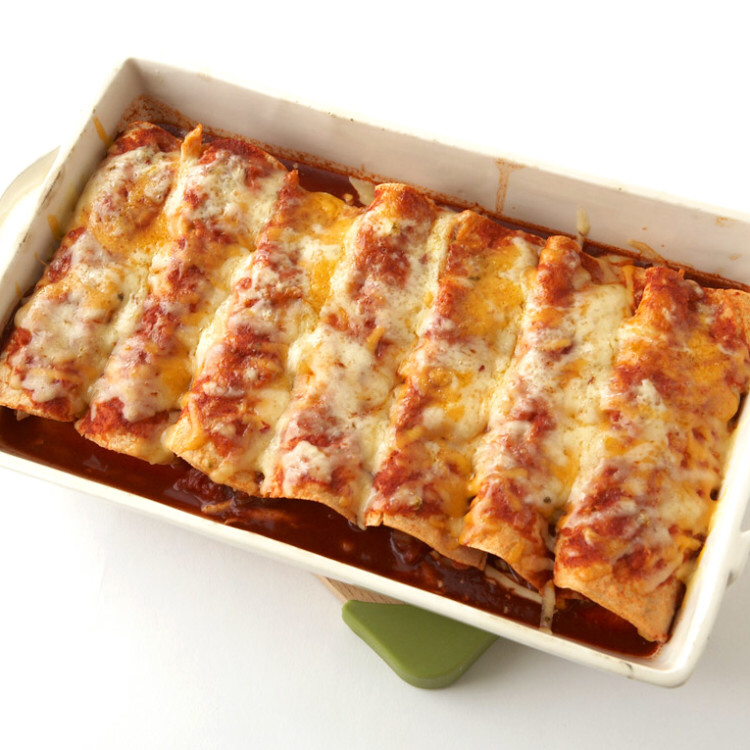
\includegraphics[height=10cm, width=8cm]{Pictures/Chicken_Enchilada.png}
\end{multicols}

\instructions
\begin{enumerate}
    \item Coat large saute pan with oil. Season chicken with salt and pepper. Brown chicken over medium heat, allow 7 minutes each side or until no longer pink. Sprinkle chicken with cumin, garlic powder and Mexican spices before turning. Remove chicken to a platter, allow to cool.
    \item Saute onion and garlic in chicken drippings until tender. Add corn and chiles. Stir well to combine. Add canned tomatoes, saute 1 minute.
    \item Pull chicken breasts apart by hand into shredded strips. Add shredded chicken to saute pan, combine with vegetables. Dust the mixture with flour to help set.
    \item Microwave tortillas on high for 30 seconds. This softens them and makes them more pliable. Coat the bottom of 2 (13 by 9-inch) pans with a ladle of enchilada sauce. Using a large shallow bowl, dip each tortilla in enchilada sauce to lightly coat. Spoon 1/4 cup chicken mixture in each tortilla. Fold over filling, place 8 enchiladas in each pan with seam side down. Top with remaining enchilada sauce and cheese.
    \item Bake for 15 minutes in a preheated \temp{350} oven until cheese melts. Garnish with cilantro, scallion, sour cream and chopped tomatoes before serving. Serve with Spanish rice and beans.
\end{enumerate}

%%% STUFFED PEPPERS %%%

\recipe{Stuffed Peppers}
\preptime{20 min}
\cooktime{1 hr}

\begin{multicols}{2}
\ingredients
\begin{itemize}
    \item 1 lb ground beef
    \item 1/2 cup uncooked long grain white rice
    \item 1 cup water
    \item 6 green bell peppers
    \item 2 (8 oz) cans tomato sauce
    \item 1 tbsp Worcestershire sauce
    \item 1/4 tsp garlic powder
    \item 1/4 tsp onion powder
    \item salt and pepper to taste
    \item 1 tsp Italian seasoning
\end{itemize}

\vfill\null
\columnbreak

\hspace{-0.7cm}
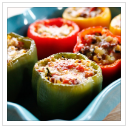
\includegraphics[height=7.25cm, width=8cm]{Pictures/Stuffed_Peppers.png}
\end{multicols}

\instructions
\begin{enumerate}
    \item Preheat oven to \temp{350}.
    \item Place the rice and water in a saucepan, and bring to a boil. Reduce heat, cover, and cook 20 minutes. In a skillet over medium heat, cook the beef until evenly browned.
    \item Remove and discard the tops, seeds, and membranes of the bell peppers. Arrange peppers in a baking dish with the hollowed sides facing upward. (Slice the bottoms of the peppers if necessary so that they will stand upright.)
    \item In a bowl, mix the browned beef, cooked rice, 1 can tomato sauce, Worcestershire sauce, garlic powder, onion powder, salt, and pepper. Spoon an equal amount of the mixture into each hollowed pepper. Mix the remaining tomato sauce and Italian seasoning in a bowl, and pour over the stued peppers.
    \item Bake 1 hour in the preheated oven, basting with sauce every 15 minutes, until the peppers are tender.
\end{enumerate}

%%% LEMON GARLIC SALMON %%%

\recipe{Lemon Garlic Salmon}
\preptime{5 min}
\cooktime{25 min}

\begin{multicols}{2}
\ingredients
\begin{itemize}
    \item 2 tbsp butter
    \item 2 tsp garlic (minced)
    \item 1 tsp lemon pepper
    \item 2 (4 ounce) fillets salmon
    \item 1 lemon
\end{itemize}

\vfill\null
\columnbreak

\hspace{-2.5cm}
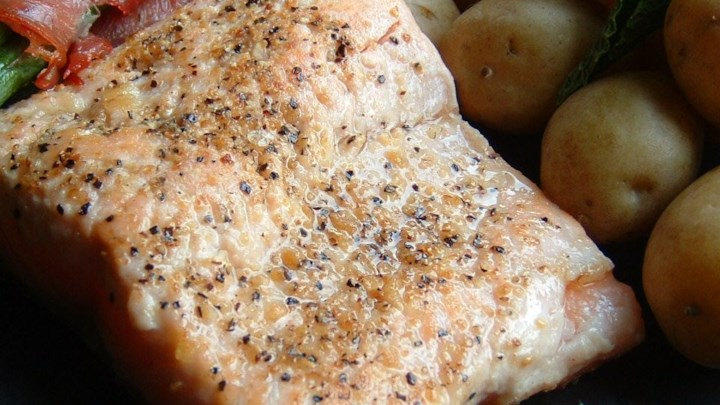
\includegraphics[height=10cm, width=10cm]{Pictures/Lemon_Garlic_Salmon.jpg}
\end{multicols}

\instructions
\begin{enumerate}
    \item Season salmon fillets on both sides with lemon pepper.
    \item In a large skillet, melt butter over medium high heat. Stir in garlic. Place salmon in pan. Cook for 10 minutes per inch of thickness, or until fish flakes when tested with a fork. Flip fillets halfway through cooking to brown on both sides. Sprinkle with lemon juice before serving.
\end{enumerate}

%%% Grilled Chicken Spice Rub %%%

\recipe{Grilled Chicken Spice Rub}
\preptime{5 min}
\cooktime{12 min}

\begin{multicols}{2}
\ingredients
\begin{itemize}
    \item 3 chicken breasts
    \item 1 tsp of garlic powder
    \item 1 tsp of ground cumin
    \item 1/2 tsp of ground coriander
    \item 1/2 tsp of smoked paprika
    \item 1/2 tsp of salt
    \item 1/4 tsp of ground black pepper
    \item 2 tbsp of olive oil    
\end{itemize}

\vfill\null
\columnbreak

\hspace{-2.5cm}
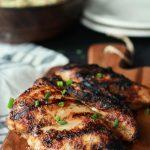
\includegraphics[height=10cm, width=10cm]{Pictures/Grilled_Chicken_Spice_Rub.jpg}
\end{multicols}

\instructions
\begin{enumerate}
    \item Preheat grill to medium high heat.
    \item In a small bowl, mix garlic powder, cumin, coriander, smoked paprika, sea salt, pepper, and olive oil. Mix until combined.
    \item Rub mixture over both sides of the chicken.
    \item Place chicken on grill and grill each side for 4-6 minutes depending on thickness. You just want to make sure there is no pink in the middle.
\end{enumerate}

%%% Oven Baked BBQ Chicken %%%

\recipe{Oven Baked BBQ Chicken}
\preptime{1 hr}
\cooktime{40 min}

\begin{multicols}{2}
\ingredients
\begin{itemize}
    \item 4 Skinless Boneless Chicken Breast Halves
    \item 3 tbsp olive oil
    \item 1 1/2 tsp smoked paprika
    \item 2 tablespoons fresh lemon juice
    \item 3 cloves garlic (minced)
    \item salt \& pepper to taste
    \item 1 cup BBQ sauce
\end{itemize}

\vfill\null
\columnbreak

\hspace{-1cm}
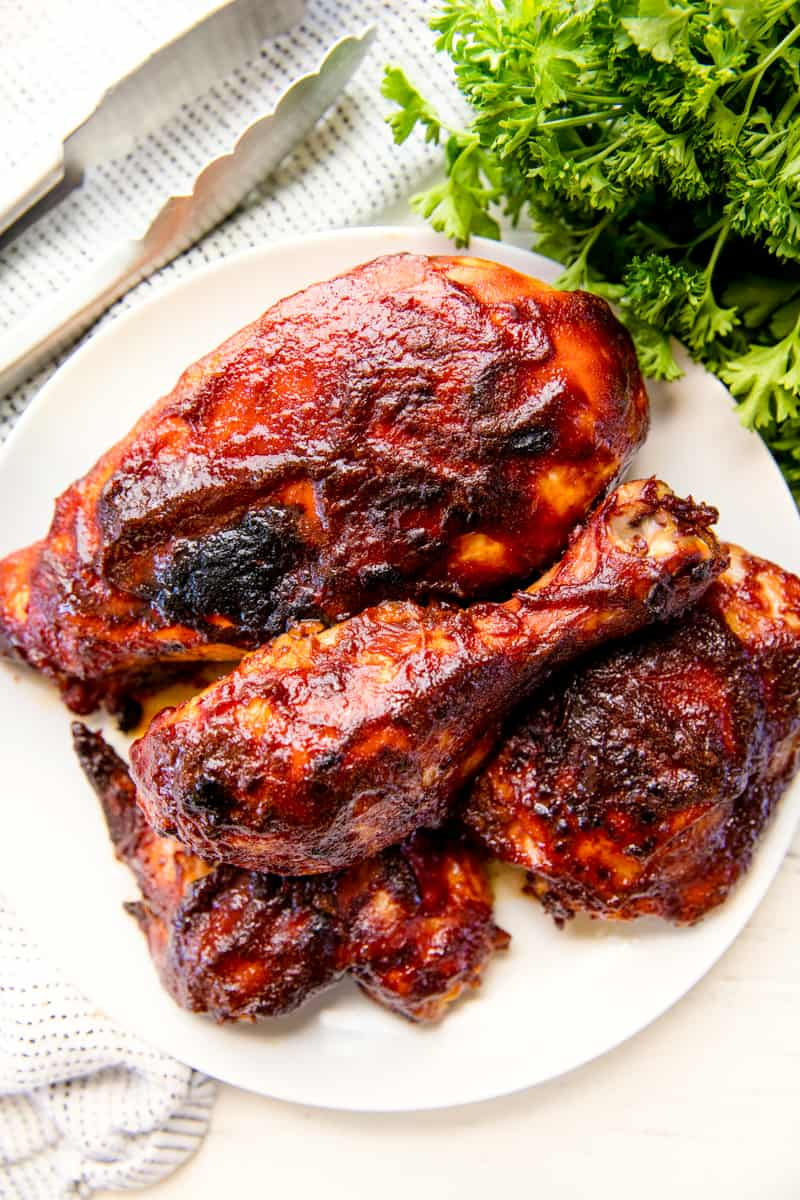
\includegraphics[height=8cm, width=8cm]{Pictures/Oven_Baked_BBQ_Chicken.jpeg}
\end{multicols}

\instructions
\begin{enumerate}
    \item Place chicken breast halves and place in a large ziplock bag.
    \item Combine olive oil, smoked paprika, lemon juice, and garlic in a small bowl and pour over chicken.
    \item Let chicken marinade for at least an hour, up to 24 hours in the fridge.
    \item Preheat oven to \temp{350}.
    \item Remove chicken from bag and place on a baking sheet. Season with salt and pepper.
    \item Bake for 20 minutes and brush a layer of BBQ sauce on the chicken. Return to the oven and repeat brushing with BBQ sauce every 5 minutes until the chicken is cooked through, about 15 to 20 minutes longer. Chicken is done when it reaches an internal temperature of \temp{165} when read with a thermometer inserted into the thickest part of the breast.
\end{enumerate}

%%% Smoked Sausage Skillet %%%

\recipe{Smoked Sausage Skillet}
\preptime{5 min}
\cooktime{15 min}

\begin{multicols}{2}
\ingredients
\begin{itemize}
    \item (14 ounce) package Smoked Sausage (cut into 1/4-inch slices)
    \item 1/4 cup olive oil
    \item 2 cloves garlic (crushed)
    \item 1 large red bell pepper (sliced thin)
    \item 1 small yellow onion (sliced thin)
    \item 1 (10 oz) package frozen broccoli (thawed)
    \item 1/2 cup chicken broth (or water)
    \item 1/2 cup tomato sauce
    \item 2 cups instant rice
    \item 1/2 cup shredded mozzarella cheese
\end{itemize}

\vfill\null
\columnbreak

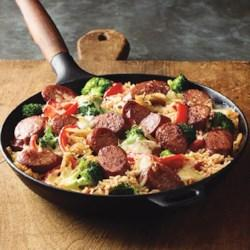
\includegraphics[height=7.5cm, width=8cm]{Pictures/Smoked_Sausage_Skillet.jpg}
\end{multicols}

\instructions
\begin{enumerate}
    \item Heat olive oil and crushed garlic, stir in smoked sausage slices and cook until smoked sausage is browned.
    \item Add pepper, onion, broccoli, chicken broth and tomato sauce and simmer for about 10 minutes until vegetables are tender and the liquid is absorbed.
    \item In the meantime, cook rice according to package instructions. Stir rice into the skillet, sprinkle with cheese and
\end{enumerate}
\end{document}
